\section{Ekstrema, hjørnepunkter og basale løsninger}
%
%\textit{Vis at løsningerne findes i hjørnene af en polytede.}
Som det fremgår i afsnit \ref{heeeeejjulle}, vil en optimal løsning oftest ligge i et hjørne på et polyeder.
Det er derfor hensigtsmæssigt at definere disse hjørner.
%
\begin{defn}{}{ekstrema}
Lad $\mathcal{P}$ være et polyeder. 
En vektor $\mathbf{u} \in \mathcal{P}$ kaldes et \textbf{ekstremumspunkt} i $\mathcal{P}$, hvis der ikke eksisterer to vektorer $\mathbf{v},\mathbf{w} \in \mathcal{P}$, $\mathbf{v} \land \mathbf{w} \neq \mathbf{u}$, samt en skalar $\lambda \in [0,1]$, hvorom det gælder, at $\mathbf{u}=\lambda\mathbf{v}+(1-\lambda)\textbf{w}$.
\end{defn}
\noindent
%
Et hjørne kan beskrives ud fra \ref{defn:ekstrema}, idet der, såfremt $\mathbf{u}=\lambda\mathbf{v}+(1-\lambda) \mathbf{w}$, og alle vektorene findes i $\mathcal{P}$, gælder, at $\mathbf{u}$ er en konveks kombination af $\mathbf{v}$ og $\mathbf{w}$.
Hvis $\mathbf{u}=\lambda \mathbf{v}+(1-\lambda) \textbf{w}$ og $\mathbf{u}$ er et ekstremumspunkt, må det derfor gælde, at $\mathbf{v}\notin \mathcal{P}$ eller $\mathbf{w}\notin \mathcal{P}$ eller $\mathbf{u}=\mathbf{w}$ eller $\mathbf{u}=\mathbf{v}$.
Bemærk, at \ref{defn:ekstrema} er strengt geometrisk. 
% Kun gælder som geometrisk definition gælder ikke som algebrarisk definition xD
På figur \ref{fig:ekstrema} ses et polyeder $\mathcal{P}$, hvor $\textbf{x}$ er et ekstremumspunkt, da der ikke findes vektorer $\textbf{y}$ og $\textbf{z}$, sådan at $\mathbf{x}=\lambda\mathbf{y}+(1-\lambda) \mathbf{z}$.
Vektor $\textbf{w}$ er derimod ikke et ekstremumspunkt, da der findes $\textbf{v}$ og $\textbf{u}$, sådan at $\mathbf{w}=\lambda\mathbf{v}+(1-\lambda)\textbf{u}$.
%

\begin{figure}[h!]
  \centering
  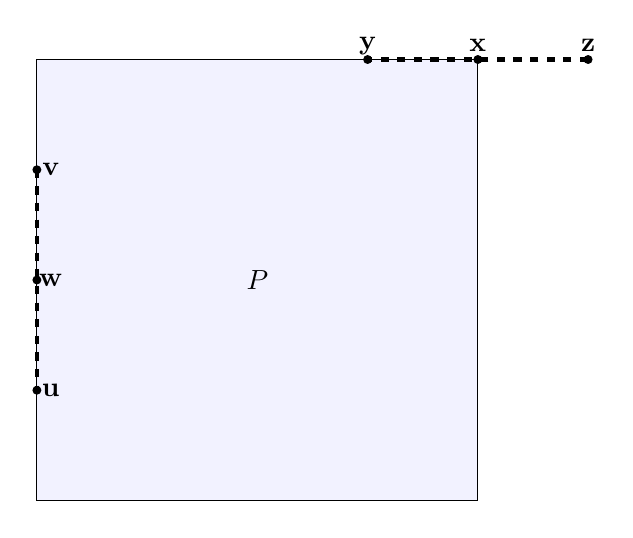
\begin{tikzpicture}[scale=0.7]
    \tikzset{punkt/.style={point, draw=black}}
    
    
%Punkter

	\node at (4,4)	(1){};
	\node at (-4,4)	(4){};
	\node at (4,-4)	(2){};
	\node at (-4,-4) (3){};


	\filldraw[black, fill=blue!5] (2) rectangle (4);
	\node at (0,0) (P){$P$};
	
	\filldraw [black] (2,4) circle (2pt);
	\filldraw [black] (4,4) circle (2pt);
	\filldraw [black] (6,4) circle (2pt);
	\filldraw [black] (-4,2) circle (2pt);
	\filldraw [black] (-4,0) circle (2pt);
	\filldraw [black] (-4,-2) circle (2pt);	
	\node at (2,4.25)	 (y){$\textbf{y}$};
	\node at (4,4.25)	 (x){$\textbf{x}$};
	\node at (6,4.25)	 (z){$\textbf{z}$};
	\node at (-3.75,2)  (v){$\textbf{v}$};
	\node at (-3.75,0)	 (w){$\textbf{w}$};
	\node at (-3.75,-2) (u){$\textbf{u}$};


	\draw[-, dashed,black,ultra thick] (6,4) -- (2,4);
	\draw[-, dashed,black,ultra thick] (-4,2) -- (-4,-2);

  \end{tikzpicture}
  \caption{En afgrænset polytop $P$ hvor $\textbf{x}$ er et ekstramapunkt da der ikke findes vektorer $\textbf{y}$ og $\textbf{z}$ sådan at $\mathbf{x}=\lambda\mathbf{y}+(1-\lambda)z$. $\textbf{w}$ er i modsætning ikke et ekstremapunkt da der findes $\textbf{v}$ og $\textbf{u}$ sådan at $\mathbf{w}=\lambda\mathbf{v}+(1-\lambda)u$.}
  \label{fig:ekstrema}
\end{figure}
%
%
%    \node[punkt] at (-4,0.5)      (v1){$v_1$};
%    \node[punkt] at (-2,0.5)      (v2){$v_2$};
%    \node[punkt] at (-4,-1.5)     (v3){$v_3$};
%    \node[punkt] at (-2,-1.5)     (v4){$v_4$};
%    \node at (-3,2)     (v){$K_{4}$};
%
%
%    \node[punkt] at (4.6,-0.2)      (k1){$v_3$};
%    \node[punkt] at (1.4,-0.2)      (k2){$v_2$};
%    \node[punkt] at (2,-2)     (k3){$v_4$};
%    \node[punkt] at (4,-2)     (k4){$v_5$};
%    \node[punkt] at (3,1)      (k5){$v_1$};
%    \node at (3,2)      (k){$K_{5}$};
%
%
%
%
%
%    \draw [-, thick, draw=black] (v1) -- (v2);
%    \draw [-, thick, draw=black] (v1) -- (v3);
%    \draw [-, thick, draw=black] (v1) -- (v4);
%    \draw [-, thick, draw=black] (v2) -- (v3);
%    \draw [-, thick, draw=black] (v2) -- (v4);
%    \draw [-, thick, draw=black] (v3) -- (v4);
\\\\
%
En alternativ geometrisk definition relaterer sig til \textit{hjørnepunkter}.
For et givet lineært programmeringsproblem er den optimale løsning i et af hjørnepunkterne.
%
\begin{defn}{}{hjoerner}
Lad $\mathcal{P}$ være et polyeder. 
En vektor $\mathbf{u}\in \mathcal{P}$ siges at være et \textbf{hjørnepunkt}, hvis der eksisterer en vektor $\mathbf{c}$, hvorom det gælder, at $\mathbf{c}^T\mathbf{u}<\mathbf{c}^T\mathbf{v}$ for alle $\mathbf{v}$, som opfylder $\mathbf{v} \in \mathcal{P}$ samt $\mathbf{v}\neq\mathbf{u}$.
\end{defn}
\noindent
%
På figur \ref{fig:julieermegaseeeeeeeeeej} ses et eksempel på et polyeder $\mathcal{P}$, hvor $\textbf{x}$ er et hjørnepunkt, da det er det eneste punkt, som både er i hyperplanet og $\mathcal{P}$.
Vektoren $\textbf{w}$ er i modsætning ikke et hjørnepunkt, da hyperplanet skærer $\mathcal{P}$ i flere punkter end $\mathbf{w}$.
%
\input{fig/tikz/geometri/hjorne}
\\\\